%\documentclass[english,10pt,handout]{beamer}
\documentclass[english,10pt]{beamer}







 
%\usepackage{mathptmx}
%\renewcommand{\sfdefault}{lmss}
\usepackage[T1]{fontenc}
%\usepackage[latin9]{inputenc}
\usepackage[utf8]{inputenc}

\synctex=-1

\usefonttheme{professionalfonts}

%\setbeamertemplate{navigation symbols}{}
%\setbeamertemplate{caption}[numbered]


\useinnertheme{rectangles}
%http://tex.stackexchange.com/questions/11168/change-bullet-style-formatting-in-beamer

 \AtBeginDocument{
  \addtolength\abovedisplayskip{-0.4\baselineskip}%
  \addtolength\belowdisplayskip{-0.4\baselineskip}%
}%change the space between text lines and the math formula


\usepackage{pifont}
%Postscript ZipfDingbats font
%the command \ding{number}, will print the specified symbol

\usepackage{fontawesome}
%icon package
\DeclareFontFamily{U}{FontAwesomeOne}{}
\DeclareFontShape{U}{FontAwesomeOne}{m}{n}{<-> FontAwesome--fontawesomeone}{}
\DeclareRobustCommand\FAone{\fontencoding{U}\fontfamily{FontAwesomeOne}\fontseries{m}\fontshape{n}\selectfont}
\DeclareFontFamily{U}{FontAwesomeTwo}{}
\DeclareFontShape{U}{FontAwesomeTwo}{m}{n}{<-> FontAwesome--fontawesometwo}{}
\DeclareRobustCommand\FAtwo{\fontencoding{U}\fontfamily{FontAwesomeTwo}\fontseries{m}\fontshape{n}\selectfont}
\DeclareFontFamily{U}{FontAwesomeThree}{}
\DeclareFontShape{U}{FontAwesomeThree}{m}{n}{<-> FontAwesome--fontawesomethree}{}
\DeclareRobustCommand\FAthree{\fontencoding{U}\fontfamily{FontAwesomeThree}\fontseries{m}\fontshape{n}\selectfont}

%ftp://ftp.dante.de/tex-archive/fonts/fontawesome/doc/fontawesome.pdf
%http://tug.ctan.org/info/symbols/comprehensive/symbols-a4.pdf


\usepackage{amsmath,amssymb,amsfonts,bm,mathrsfs,mathtools}

\usepackage{tikzsymbols}
%\usepackage[tikz]{bclogo}



\usepackage{perpage}
\MakePerPage{footnote} %reset for each page
%\renewcommand{\thefootnote}{\fnsymbol{footnote}} %use symbol, limit less than 9 symbols



%%%% HIGHTLIGHT  and annotation &=%%%%%%%%
\usepackage{color,xcolor}
 \usepackage{todonotes}

\usepackage[normalem]{ulem}

\usepackage[many]{tcolorbox}

\tcbset{fonttitle=\scriptsize}
\tcbset{highlight math style={enhanced,
  colframe=red!40!black,colback=yellow!20!white,arc=2pt,boxrule=.2pt,
  }}
  \newtcbox{\otherbox}[1][]{nobeforeafter,math upper,tcbox raise base,
enhanced,frame hidden,boxrule=0pt,interior style={top color=green!10!white,
bottom color=green!10!white,middle color=green!50!yellow},
fuzzy halo=1pt with green,#1}
%%\tcbhighmath{math here}
%% \otherbox{math here}



%%%%% HIGHLIGHT %%%%%%
\newcommand{\hb}[1]{{\color{blue}{#1}}}
%\noindent\rule{\textwidth}{.5pt}

%:
\usepackage{soul}

\newcommand\hcancel[2][black]{\setbox0=\hbox{$#2$}%
\rlap{\raisebox{.45\ht0}{\textcolor{#1}{\rule{\wd0}{1pt}}}}#2}
%cross to delete

\newcommand{\mcb}[2]{\colorbox{#1}{$\displaystyle #2$}}
%highlight math

\newcommand{\hlfancy}[2]{\sethlcolor{#1}\hl{#2}}
%specified color , for\hl

\newcommand\myhl{\bgroup\markoverwith
  {\textcolor{yellow}{\rule[-.5ex]{2pt}{2.5ex}}}\ULon}



\mode<presentation>{ \usetheme{boxes} }

%write Matlab code
\usepackage{listings}
 \definecolor{dkgreen}{rgb}{0,0.6,0}
\definecolor{gray}{rgb}{0.5,0.5,0.5}
\definecolor{mauve}{rgb}{0.58,0,0.82}
\lstset{frame=tb,
  language=Matlab,
  aboveskip=3mm,
  belowskip=3mm,
  showstringspaces=false,
  columns=flexible,
  basicstyle={\small\ttfamily},
  numbers=none,
  numberstyle=\tiny\color{gray},
  keywordstyle=\color{blue},
  commentstyle=\color{dkgreen},
  stringstyle=\color{mauve},
  breaklines=true,
  breakatwhitespace=true
  tabsize=3
}

\usepackage[lastexercise]{exercise}

\newtheorem{ex}{Exercise}
\newtheorem{property}{Property}
\newtheorem{ag}{Algorithm}
\newtheorem{remark}{Remark}
\newtheorem{den}{definition}
\newtheorem{assumption}{Assumption}


\usepackage[nosolutionfiles]{answers}
\Newassociation{sol}{Solution}{ans}



\usepackage{empheq}
\usepackage{comment}
%\usepackage{lscape}
\usepackage{multirow}
\usepackage{url,hyperref}

\hypersetup{
 %   bookmarks=true,         % show bookmarks bar?
    unicode=false,          % non-Latin characters in Acrobat's bookmarks
    pdftoolbar=true,        % show Acrobat's toolbar?
    pdfmenubar=true,        % show Acrobat's menu?
    pdffitwindow=false,     % window fit to page when opened
    pdfstartview={FitH},    % fits the width of the page to the window
    pdftitle={My title},    % title
    pdfauthor={Author},     % author
    pdfsubject={Subject},   % subject of the document
    pdfcreator={Creator},   % creator of the document
    pdfproducer={Producer}, % producer of the document
    pdfkeywords={keyword1} {key2} {key3}, % list of keywords
    pdfnewwindow=true,      % links in new window
    colorlinks=true,       % false: boxed links; true: colored links
    linkcolor=red,          % color of internal links (change box color with linkbordercolor)
    citecolor=green,        % color of links to bibliography
    filecolor=magenta,      % color of file links
    urlcolor=cyan           % color of external links
}


\usepackage{subfigure,epsfig,graphicx,graphics}

\DeclareGraphicsRule{.tif}{png}{.png}{`convert #1 `dirname #1`/`basename #1 .tif`.png}
   \DeclareGraphicsExtensions{.pdf}




\newcommand{\hw}{ {\underline{\tt Homework }} }
\newcommand{\hws}{ {\underline{\tt Homework$\star$}} }
\newcommand{\optional}{ {\it optional} }

\newcommand{\MATLAB}{ \texttt{MATLAB}}
\newcommand{\python}{ \texttt{python}}
\newcommand{\Rlang}{ \texttt{R}}
\newcommand{\SAS}{ \texttt{SAS}}
\newcommand{\MC}{Markov Chain}


\newcommand{\tm}{transition matrix}
\newcommand{\rv}{random variable}
\newcommand{\spl} {supervised learning }
 

\newcommand{\dis}{\underline{\tt discussion}: }
\newcommand{\pri}{\underline{\tt principle}: }




\newcommand{\bq}{\scalebox{6}{\textbf{?} }}
\newcommand{\sq}{\scalebox{2}{\textbf{?} }}
\newcommand{\ck} {  {\scalebox{0.8} {\Interval}   } }

\newcommand{\eps}{\varepsilon}
\newcommand{\To}{\longrightarrow}

% 
\newcommand{\Dcal}{\mathtt{D}}
\newcommand{\Hcal}{\mathcal{H}}
\newcommand{\Ecal}{\mathcal{E}}
\newcommand{\Xcal}{\mathcal{X}}
\newcommand{\Ycal}{\mathcal{Y}}
\newcommand{\Zcal}{\mathcal{Z}}

%%Calculus 

\renewcommand{\d}{\ensuremath{\mathrm{d}}}
\newcommand{\dt}{ \ensuremath{\mathrm{d} t } }
\newcommand{\dx}{ \ensuremath{\mathrm{d} x} }
\newcommand{\dy}{ \ensuremath{\mathrm{d} y } }

%indicator function
\newcommand{\indf}{ \ensuremath{\mathbf{1} } }



%probability
\newcommand{\p}{ \mathbb{P}}
\newcommand{\prob}{{\Pr}}
\newcommand{\PP}{\mbox{PP}}%Poisson process
%condition prob
\newcommand{\cPr}[2]{{\Pr\left(#1\mid #2\right)}}

\newcommand{\FF}{{\mathbb{F}}}

\newcommand{\e}{ \operatorname{\mathbb E}}
\newcommand{\Var}{\operatorname{\mathbb{V} }}
\newcommand{\var}{\operatorname{\text{Var} }}
\newcommand{\MSE}{\operatorname{\text{MSE} }}

\newcommand{\Std}{\operatorname{std}}
\newcommand{\Cov}{\operatorname{cov}}

%Matrix  %mathbf
\newcommand{\Pb}{{\mathbf{P}}}
\newcommand{\Qb}{{\mathbf{Q}}}
\newcommand{\Mb}{{\mathbf{M}}}
\newcommand{\cb}{\mathbf{c}}
\newcommand{\bb}{{\mathbf{b}}}

\newcommand{\Tb}{\mathbf{T}}

\newcommand{\Wb}{\mathbf{W}}
\newcommand{\wb}{\mathbf{w}}
\newcommand{\Xb}{\mathbf{X}}

\newcommand{\xb}{\mathbf{x}}

\newcommand{\Wtn}{\mathbb{W}}
\newcommand{\btn}{\mathbf{b}}



\newcommand{\eye}{{\mathbf{I}}}
%identity matrix
\newcommand{\onem}{{\mathbb{1}}}
\newcommand{\idor}{\mathbf{1}}
\newcommand{\ii}{\mathbf{i}}
%imaginary symbol

\usepackage{tikz}

%State number
\newcommand{\snum}[1]{ \raisebox{.5pt}{\textcircled{\raisebox{-.9pt} {#1}}}}

 \usetikzlibrary{arrows}
\usetikzlibrary{shapes}

%\newcommand{\snum}[1]{%
 % \tikz[baseline=(char.base)]\node[anchor=south west, draw,rectangle, rounded corners, inner sep=1.4pt, minimum size=5mm,
   % text height=1.3mm](char){\ensuremath{#1}} ;}

\newcommand*\circled[1]{\tikz[baseline=(char.base)]{
            \node[shape=circle,draw,inner sep=.4pt] (char) {#1};}}


%real number
\newcommand{\Real}{{\mathbb{R}}}
%integer
\newcommand{\ZZ}{\mathbb{Z}}
%positive integer
\newcommand{\NN}{\mathbb{N}}



\newcommand{\inpd}[2]{\left\langle #1, #2 \right\rangle}
\newcommand{\abs}[1]{\left\vert#1\right\vert}
\newcommand{\norm}[1]{\left\|#1\right\|}
\newcommand{\wt}[1]{{\widetilde{#1}}}
\newcommand{\set}[1]{\left\{#1\right\}}
\newcommand{\partiald}[2]{  \frac{\partial #1 }{\partial #2}}



\newcommand{\ie}{{\it{i.e.}}}



\newcommand{\transpose}{\textsf{T}} % or, \intercal
\newcommand{\diag}{\textsf{diag}}
\newcommand{\tr}{{\textsf{T}}}
\newcommand{\rt}{{\textbf{r}}}

\DeclareMathOperator{\trace}{Trace}


\newcommand{\argmin}{ \operatornamewithlimits{argmin} }
\newcommand{\argmax}{ \operatornamewithlimits{argmax} }




\def\biz{\begin{itemize} }
\def\bizp{\begin{itemize}[<+->] }
\def\eiz{\end{itemize}}


\def\bfm{\begin{frame}}
\def\efm{\end{frame}}

\def\bena{\begin{enumerate}[<+-| alert@+>]}
\def\ben{\begin{enumerate}}
\def\een{\end{enumerate}}


\def\bbk{\begin{block} }
\def\ebk{\end{block}}






\makeatletter
%%%%%%%%%%%%%%%%%%%%%%%%%%%%%% Textclass specific LaTeX commands.
 % this default might be overridden by plain title style

%%%%%%%%%%%%%%%%%%%%%%%%%%%%%% User specified LaTeX commands.
%\usetheme{Warsaw}
\usetheme{Boadilla}
% or ...



%\setbeamertemplate{footline}[text line]{} % makes the footer EMPTY
%\setbeamertemplate{footline}[page number]{} % makes the footer EMPTY

%\usecolortheme{orchid} %not use is better 

\setbeamertemplate{footline}[text line]{%
  \parbox{\linewidth}{\vspace*{-2pt}Xiang Zhou\hfill CityU\hfill \insertpagenumber}}
%\setbeamertemplate{navigation symbols}{}

%\setbeamercovered{transparent}
% or whatever (possibly just delete it)


%\usepackage{babel}
\makeatother



 %
%\addtobeamertemplate{frametitle}{}{%
%\begin{tikzpicture}[remember picture,overlay]
%\node[anchor=south east,yshift=2pt] at (current page.south east) {
\includegraphics[height=0.6cm]{CityU_Logo_Basic_Signature.eps}};
%\end{tikzpicture}}
%

\beamerdefaultoverlayspecification{<+->}
%the presentation acts as though a \pause command has been inserted between every two bullets, without the actual need to write \pause after each item.



\newcommand{\fv}{{\boldsymbol{f}}}
\newcommand{\gv}{{\boldsymbol{g}}}
\newcommand{\sv}{{\boldsymbol{\psi}}}
\newcommand{\pv}{{\boldsymbol{\varphi}}}
\newcommand{\Ps}{{\wt{\Pm}}}


\begin{document}

 

 

 \frame{{Chapter 2: Discrete-Time Markov Models (Part ii , iii)}
\begin{center}

\includegraphics[scale=0.4]{Markov-chain-banner.png}
\bigskip \par 
 Andrey  Markov (1856-1922, Russian mathematician)
\end{center}
}

\frame{{Part ii: Limiting Behavior of DTMC }
--- What happens if a DTMC runs for a very long time ?
}


\begin{frame}
\frametitle{Start from these (simple two-state) examples}

{What happens to  these Markov Chains as $n\to \infty$ ?}

{\small \it draw a picture, study the dynamics,  see what you get ... }

\ben
\item   $\Pm=\begin{bmatrix}
1&0\\ 0&1
\end{bmatrix} $
\item $\Pm=\begin{bmatrix}
0&1\\ 1&0
\end{bmatrix} $
\item $\Pm=\begin{bmatrix}
1&0\\ 1/2&1/2
\end{bmatrix} $
\item $\Pm=\begin{bmatrix}
1/2&1/2\\ 1/4& 3/4
\end{bmatrix} $
\een
%
\pause


Observation :  let $a^{(n)}=\p(X_n=\cdot)$ be transient distribution, then
$a^{(n)} = a^{(0)} \Pm^n$. Let $n\to \infty$. If 
$a^{(n)} \to \pi$,  then
$\pi = a^{(0)}\displaystyle \lim_{n\to\infty} \Pm^n $ 
\\

What is  $\displaystyle \lim_{n\to\infty}\Pm^n$   for these examples ?

\pause
See also 
Textbook: Example 2.15, 2.16  (page 25) 



\end{frame}

\begin{frame}
\frametitle{Limiting distribution}

\begin{definition}
[{limiting} or \textit{steady-state}  distribution]
The (row) probability vector $
\pi=[\pi_{1},\pi_{2},\cdots,\pi_{N}] $
is the limiting distribution where 
\[
\pi_{j}=\lim_{n\to\infty} \p(X_{n}=j).
\]

\end{definition}

\pause
\begin{alertblock}{Questions to answer:}
 \biz[<+->]
\item Does the limiting distribution  $\pi$  exists ? 
\item {If it exists, is it unique (for {\it any} initial distribution)?   }
\item  How can  we compute it?
\eiz
\end{alertblock}
\pause
We first derive a {\it steady-state or balance  equation} for $\pi$: a necessary condition that
$\pi$ must satisfy.
 
\end{frame}

\begin{frame}
\begin{theorem}%{}
If a limiting distribution $\pi$ exists, it satisfies the following
balancing equation

\[
\pi_{j}=\sum_{i=1}^{N}\pi_{i}p_{ij}
\]
or in matrix form

\[
\pi=\pi \Pm
\]
\end{theorem}%{}
\medskip
 The limiting distribution
$\pi$ is the left-eigenvector of $\Pm$ corresponding to eigenvalue
$1$ satisfying  the normalizing equation 
$\sum_{j=1}^{N}\pi_{j}=1.$
\pause
\begin{proof}
The $n$-step transient distribution (the law of $\{X_n\}$), $a^{(n+1)}$, satisfies 
$a^{(n+1)}=a^{(n)}{\Pm}$. Let $n\to \infty$. Since $a^{(n)}, a^{(n+1)} $ both go to $\pi$,
we have $\pi=\pi\Pm$.
\end{proof}

\pause
\bigskip 
Textbook: 
Example 2.15, 2.16  (page 25)


\end{frame}

\frame{Stationary or invariant distribution }

\begin{frame}
\begin{definition}%{}
<1-> $\mu=[\mu_{1},\mu_{2},\cdots,\mu_{N}]$ is a
\textit{stationary} (or \textit{invariant}) distribution if 
\[
\p(X_{0}=i)=\mu_{i}, \forall i \in S \, \Longrightarrow\,\p(X_{n}=i)=\mu_{i}, \forall n >0, \forall i\in S.
\]
\end{definition}%{}

It is clear that  the condition holds for $n=1$ is sufficient for $\mu$ being invariant distribution.

\medskip 
\begin{theorem}%{}
<2->A probability vector $\mu$ is a  {stationary}
distribution of the Markov chain with transition  matrix $\Pm$ \underline{if and only if}
\[
\mu=\mu \Pm.
\]

\end{theorem}%{}
 \bigskip
Textbook: 
Example 2.17, 2.18  (page 28)

\end{frame}


\begin{frame}{If the   limiting distribution $\pi$ uniquely exists, then }

\biz[<+->]
\item Since $a^{(n)}=a^{(0)}\Pm^n$, then  $\pi = a^{(0)}\lim_n\Pm^n$ and $\pi$ is independent of $a^{(0)}$. Particularly,
\biz
\item  choose $a^{(0)}=(1,0,0,\ldots, 0)$, then $\pi=$ the first row of  $\lim_n\Pm^n$
\item   choose $a^{(0)}=(0,1,0,\ldots, 0)$, then $\pi=$ the second row of  $\lim_n\Pm^n$
\item ......
\item Each row of    $\lim_n\Pm^n$ is exactly $\pi$.
\eiz
\item So, the limit $ \underset{n\to\infty}\lim\Pm^n$ must be the following very special rank-1 matrix whose each row
is the liming distribution $\pi=[\pi_1,\pi_2,\ldots,\pi_N]$.
\[
\lim_n\Pm^n =
\begin{bmatrix}
   \pi_1 & \pi_2 &  \ldots &\pi_N \\
    \pi_1 & \pi_2 &  \ldots & \pi_N \\
    \vdots\\
      \pi_1 & \pi_2 &  \ldots & \pi_N
    \\
 \end{bmatrix} =
\begin{bmatrix}
   \pi \\
   \pi \\
   \vdots
   \\
   \pi
\end{bmatrix} =\begin{bmatrix}
   1 \\
   1\\
   \vdots
   \\
   1
\end{bmatrix} \pi
=\onem \pi
\]
(note $\onem$ is column vector, $\pi$ is row vector.)
\item The balancing equation  $\pi = \pi \Pm$ has a unique non-negative solution.
\eiz



\end{frame}

\begin{frame}[fragile]
\frametitle{How to use MATLAB to solve the balancing equation?}
  Example 2.15 (page 25).
\begin{lstlisting}
>> P=[.2 .3 .5; .1 0 .9; .55 0 .45];
>> [V,D]=eig(P')  %   solve the eigenvectors  of transpose of P
V = %eigenvectors 
     -0.5726        -0.62554              	  -0.62554     
     -0.17178       0.24327 -   0.4491i      0.24327 +    0.4491i 
     -0.80164       0.38228 +   0.4491i      0.38228 -    0.4491i
D = %eigenvalues 
            1               0                    0
            0             -0.175 - 0.32307i   	 -0.175 + 0.32307i
            0               0                     0 
>> mu=V(:,1)./sum(V(:,1))     % normalise the first column 
mu =
      0.37037
      0.11111
      0.51852
\end{lstlisting}
\pause try Example 2.16 by yourself in which no limiting distribution exists, but the balancing equation still has one unique solution.
\end{frame}

\frame{{application: Markov chain with discounted reward}
Assume that $(X_n)$ is a DTMC with the transition matrix $\Pm$.
$0<\alpha<1$ is a constant. $c$ is a scalar-valued function defined on the state
space $S=\set{1,\dots,N}$.
Let 
\[
u(x)= \e \left[ \sum_{n=0}^\infty \alpha^{n} c(X_n) \vert X_0=x\right],
~~x\in S.
\]
Then show that the vector $\bm u$ satisfies the linear equation
\[\boxed{\bm u =\bm c+\alpha \Pm \bm u}\]
where $\bm u=[u(1),\ldots, u(N)]^\tr$ and $\bm c=[c(1),\ldots, c(N)]^\tr$. 
\par\bigskip {\it Proof:} $\e c(X_n\vert X_0=i)= \sum_{j\in S} c(j) \p(X_n=j\vert X_0=i)
=\sum_j (\Pm^n)_{ij} c(j) = \Pm^n \bm c$.
Then $\bm u= \sum_{n=0}^\infty \alpha^n  \Pm^n \bm c =
(\eye-\alpha\Pm)^{-1} \bm c$, which is 
$\bm u + \alpha \Pm \bm u=\bm c$.
}

\frame{Occupancy Distribution: frequency of time when DTMC visited a given state}
\begin{frame}
\begin{definition}%{}
The occupancy distribution $\nu=[\nu_1,\nu_2,\cdots,\nu_N]$ is 
\[\nu_{j}=\lim_{n\to\infty}\frac{\e\left(N_{j}^{(n)}\: \vert ~ X_{0}=i\right)}{n+1}.
\]
%=\lim_{n\to\infty}\frac{ m_{i,j}^{(n)} }{n+1}
\end{definition}%{}
(formally  $\nu_j$     depends on the initial $i$ from this def.)

\biz[<+->]
\item
Recall  that $N_j^{(n)}=\sum_{t=0}^n 1_{\{X_t=j\}} $ 
and $m_{i,j}^{(n)}=\e (N_j^{(n)}|X_0=i)$ is the occupancy time up to $n$ of state $j$ starting from
state $i$.


\item
It is clear that $\sum_{j\in S}\nu_{j}=1$ since $\sum_{j\in S} 1_{\{X_t=j\}} = 1$.
\item
By [Thm 2.4] ($\Mm^{(n)}=\sum_{t=0}^n \Pm^{t}$), the connection to the transition matrix is 
\[ \nu_{j}=\lim_{n\to\infty}\frac{ m_{i,j}^{(n)} }{n+1}
= \lim_{n\to\infty} \frac{ 1}  {n+1} \sum_{t=0}^np^{(t)}_{ij}  \]
where $p^{(t)}_{ij}=(\Pm^t)_{i,j}$ is the $(i,j)$
of the $t$-step transition matrix.
\eiz


\end{frame}



\frame
{


 \begin{theorem}[Thm 2.7]
If the occupancy distribution $ \nu$ exists, then it satisfies
the  balance and normalizing equations: 
\[
\nu = \nu \Pm,  
~~~~~~~~~~
\sum_{j \in S}\nu_{j}=1.
\]
\end{theorem}{\it Proof:}\footnote{  textbook page 29.} 
\vspace {-15pt}
\[
\begin{split}
 \nu_{j}&=\lim_{n\to\infty}\frac{ m_{i,j}^{(n)} }{n+1}
= \lim_{n\to\infty} \frac{ 1}  {n+1} \sum_{t=0}^n  p^{(t)}_{i,j}\\
&=\lim_{n\to\infty} \frac{ 1}  {n+1}
\left(  p^{(0)}_{ij}  +\sum_{t=1}^n  p^{(t)}_{i,j} \right)
\\
&=\lim_{n\to\infty} \frac{ 1}  {n+1}
\left(  p^{(0)}_{ij}+\sum_{t=1}^n \sum_{k\in S} p^{(t-1)}_{i,k} p_{k,j} \right)
(\because \mbox{C-K eqn.})
\\
&=\lim_{n\to\infty} \frac{ n}  {n+1}
  \sum_{k\in S} \frac{1}{n}\sum_{t=0}^{n-1}   p^{(t)}_{i,k} p_{k,j} 
  \\
  &=
  \sum_{k\in S}  {\color{blue}{\lim_{n\to\infty} \frac{1}{n}\sum_{t=0}^{n-1}   p^{(t)}_{i,k}}} p_{k,j} \\
  &= \sum_{k\in S}  \nu_k p_{k,j}
\end{split}
\]


}



\begin{frame}
\frametitle
{Application:  Section $2.6.2$ Long-Run Expected Cost Rate  }

Let $c(x)$ be a cost function. The expected long-run cost rate is defined as 
\[  \mathcal{C}_i  \triangleq \lim_{n\to\infty}\frac{1}{n+1}\e \left[ \sum_{t=0}^nc(X_t)\vert X_0=i\right]. \]
Its calculation derived below leads to  Theorem 2.12 (page 38). By  Thm 2.11 and the definition of $\nu$,
\[
\begin{split}
\mathcal{C}_i &=\lim_{n\to\infty} \sum_{j\in S} \frac{1}{n+1} c(j) m^{(n)}_{ij}   
\\
&= \sum_{j\in S}c(j) \nu_j \qquad  \mbox{       (indepenent of } i )
\end{split}
\]
which is the expectation of the   function $c$ under the occupancy distribution: 
\[\boxed{ \mathcal{C} = \e_{\nu} (c)}\]
{\bf Remark:}\footnote{\optional}
A stronger property (``strong ergodicity'') is that:
the empirical measure 
$ \frac{1}{n+1}\sum_{t=0}^{n} \delta_{X_t}(\cdot) $
(which is {\it random})
weakly 
converges to a unique  probability measure $\nu$: as $n\to \infty$,
$\frac{1}{n+1}\sum_{t=0}^{n} c({X_t})\to   \e_{\mu}[c] := \sum_{x\in S }c(x) \nu(x)$.
\end{frame}

\frame{{  Theories}
Existence/Uniqueness of $\pi, \mu,\nu$ ?  
\pause
\par
\it{ depends on the structure of the transition diagram}}

 \begin{frame}
\biz[<+->]
\item
Why the very simple DTMC  $\Pm=\begin{bmatrix} 1 & 0 \\
0 & 1 \end{bmatrix}$ does not have a unique limiting distribution?
The transient distribution $a^{(n)}=a^{(0)} \eye^n=a^{(0)}$ is unchanged at all! 
 state 1 does not talk to state 2; state 2 does not talk to state 1, either.  --- 
No communication, no mixing of the initial distribution.
 \item (unique) limiting distribution should  {\emph {forget}} any information of the initial state
and uniquely exists: 
wherever the DTMC starts,  the process should converge to the same destination.
\eiz
\pause
\begin{definition}
A state $j$ is said to be {\bf accessible} from a state $i$ (written $i\rightarrow j$)  if 
there is an  $n {\color{blue}\geq} 0$ such that 
\vspace{-2pt}
\[
\p(X_{n}=j\,\vert X_{0}=i)=(\Pm^n)_{ij}>0.
\]
A state $ i$ is said to {\bf communicate} with state $j$ (written $ i \leftrightarrow j$) if both  $i \rightarrow j$ and $j \rightarrow i$.
\end{definition}
\par
$i\rightarrow j$ means that 
it is possible (i.e. with nonzero probability) to go from     $i$ to    $ j$   in one or more steps or, alternatively, there is a directed path from   node $i$ to   node $j$ in the transition diagram of the DTMC. \par
  

\end{frame}

\begin{frame}

{\bf Properties of ``$\leftrightarrow$'' relationship} 
\biz[<+->]
 \item $n\geq 0$ implies that $n$ could be $0$, thus $i\leftrightarrow i$ for any state $i$. (Reflexivity)

\item if $i\leftrightarrow j$, then $j\leftrightarrow i$. (Symmetry)
\item if $i\to j$ and $j\to k$, then $i\to k$  (Transitivity),
and if $i\leftrightarrow j$ and $j\leftrightarrow k$, then $i\leftrightarrow k$. 
(exercise: prove this claim)
 \eiz
 
 \pause 

\bigskip
 {\bf Remark:} for each state $i$, we can define  its  {\bf communicating class}:
 \[ [i]:=\set{j\in S:  i\leftrightarrow j} \]
Note $[i]=[j]$ if and only if $i\leftrightarrow j$.
\pause
 Therefore the relation ``$\leftrightarrow$'' is a called an 
 {\bf equivalence relation} and it induces a partition of the state space $S$ into disjoint subsets 
 $S_1,\ldots, S_K$ such that 
 \[S = S_1 \cup \ldots \cup S_K \]
 and any two states communicate if and only if they are in the same subset.
 The sets  $S_1,\ldots, S_K$ are called the {  communicating classes} of the chain.
 \par
 If there is only one communicating class, i.e., $S$ itself,
 then we call this chain is  {\bf irreducible};
 Otherwise, we call it {\bf reducible }   since it can be ``reduced'' to multiple  communicating classes.
 
\end{frame}


%\frame{Irreducible DTMC}
\begin{frame}

\begin{definition}%{}
A DTMC ${X_{n},n\geq0}$ on state space $S=\{1,2,\cdots,N\}$ is said
to be \textbf{irreducible} if  its {\it any} two states communicate, \ie, $i\leftrightarrow j, \forall i,j 
\in S$% ($i=j$ is allowed).
% in other words,   if its state space is a {\it single} communicating class connected by the paths
 %in  the transition diagram.

A DTMC that is not irreducible is called reducible.
\end{definition}%{}


A chain  is   irreducible if for any two states $i,j$, there exists an integer $n$(possibly depending on $i$ and $j$) such that $(\Pm^{n})_{ij}  > 0$. 

\pause
 
\begin{theorem}[ Thm2.8, 2.9 (Ergodicity Theorems)]
If a \underline{finite-state}  DTMC is irreducible, then

\begin{enumerate}
\item its stationary distribution $\mu$  uniquely exists.
\item its occupancy distribution $\nu$ uniquely exists.
\item $\mu=\nu$, which is  the unique solution of the balance equation (together with normalizing equation and non-negativity  for probability vector).
\item $\mu_i>0,\forall i \in S$ \end{enumerate}
\end{theorem}%{}
\pause
Remark: The last property is called  positive recurrent, which may  not hold true if the state space $S$ is  infinite.  

\note{Actually this is a corollary from   Perron-Frobenius theorem for irreducible matrices.}
\pause
{{\bf Ergodicity} $:$ time average ( occupancy distribution $\nu$ ) = ensemble average (stationary distribution $\mu$ )}


\end{frame}


\begin{frame}
\frametitle{ What about   limiting distribution? : aperiodicity}
\biz[<+->]
\item Why the   {\it irreducible } DTMC  $\Pm=\left[\begin{matrix} 0 & 1 \\
1& 0 \end{matrix}\right]$  still does not have a limiting distribution ?
($\Pm^{2n}=\eye, \Pm^{2n+1}=\Pm$).
 state 1 and 2 do  communicate. But state 1(or 2) returns to itself at every two steps.
\item This DTMC is periodic with period 2.
\eiz
\pause 
\begin{definition}
A state $i$ has period $d$ if any return to state $i$ must occur in multiples of $d$   steps. Formally, the period of a state is defined as
\[ d = \operatorname{gcd}\big\{ n \geq 1: \p(X_n = i | X_0 = i) > 0\big\} \]
(where "gcd" is the greatest common divisor).
If $d=1$, then the state i is said to be {\bf aperiodic}.
\end{definition}
\bigskip 

 
Refer to Example 2.21, 2.22, page 31.
\end{frame}

\begin{frame}
It is possible that $$\big\{ n \geq 1: \p(X_n = i | X_0 = i) > 0\big\} $$ is an empty set! 
{\small
Consider the example $
\Pm=\left(\begin{array}{cc}
0 &1\\
0 &1\\
\end{array}\right)
$. Then $  \p(X_n = 1 | X_0 = 1) = 0 $ for any $n \geq 1$
since $\Pm^n= \Pm$ for any $n\geq 1$.
In this (degenerate) case of empty set, 
we say the period of the state $1$ is $0$.
 }
\pause 


It can be  proved (by elementary number theory\footnote{optional: Refer to details at 
\url{http://www.mathematik.uni-ulm.de/stochastik/lehre/ss06/markov/skript_engl/node12.html}
(Thm 2.8,2.9 therein)}) that 
\ben
\item a state $i$ is aperiodic if and only if there exists $ 0\leq n <+\infty$ such that for  {\bf all} $k \geq n$,
$ \p(X_{k} = i | X_0 = i) > 0$ , \ie, $(\Pm^{k})_{ii}>0$.
\item
If $i \leftrightarrow j$, then $i$ and $j$ have the same period.
\een

\pause
\begin{definition}
All states in one communicating class share the same period;
This period is then called as the period of the communicating class.
All states in an {\it irreducible} DTMC share the same period, which 
is also called as the period of this irreducible DTMC.
\end{definition}


\end{frame}

\begin{frame}\par
{\small
{proof:}\footnote{{\optional}} (2). 
\biz
\item
If $i=j$, the conclusion is trivial. Now we assume $i\neq j$.

Denote $A_j := \{n\geq 1: X_n=j | X_0=j\}$.
 Let $d_i$, $d_j$ be the period of state $i$, $j$, respectively.
 Since $i \leftrightarrow j $,
then there exit two integers $k_1, k_2$ such that $(\Pm^{k_1})_{ij}>0$
and  $(\Pm^{k_2})_{ji}>0$, and $k_1\geq 1,k_2\geq 1$ since $i\neq j$.
 This fact implies that $k_1+k_2$ (or $k_2+k_1$) belongs to both $A_i$ and $A_j$.
 (why? C-K eqn.)
 
\item  We claim  that if  $A_i$ is empty, then $A_j$ is empty too.
If not so, then there is $m\in A_j$, i.e.,   
  $ (\Pm^m)_{jj}>0$.
 So $(\Pm^{k_1+m})_{ii}\geq (\Pm)^{k_1}_{ij}(\Pm^{m})_{jj}>0$, 
 implying
 $m+k_1\in A_i$ which is a contradiction.
 \item  Now we assume neither of $A_i$ nor $A_i$ is empty.
We shall show that  any number in $A_j$   is divisible by  $d_i$.
Then by definition of ``gcd'' for $A_j$, we know $d_i\leq d_j$.  
By symmetry, it is also true that $d_j\leq d_i$. So, $d_i=d_j$. 
Here is the detail.
\par
Pick up any number $n$ from $A_j$, then   $k_1+n+k_2$   belongs to $A_i$
(consider $i\to j\to j\to i$).  So $n$ must be divisible by $d_i$
since both $k_1+n+k_2$ and $k_1+k_2$ are divisible by $d_i$
(because they are in $A_i$).

\eiz
}
\end{frame}


\begin{frame}
\begin{theorem}[Theorem 2.10 (Unique Limiting Distribution)]
 A finite-state irreducible aperiodic DTMC has a unique limiting distribution.
\end{theorem}



\end{frame}

\begin{frame}
\begin{ex}
Consider the following   DTMC:
$S=\set{1,2,3,4}$ and the transition matrix is
 $\Pm=\left[\begin{matrix} 0 & 1 &0 & 0  \\
1/2& 0 &1/3 & 1/6  \\
0 & 0 & 1 & 0 \\
0 & 0& 1/2 &1/2 \end{matrix}\right].$ 
\end{ex}

There are three communication classes $\set{1,2}$   $\set{3}$ and  $\set{4}$.
The solution of the balance equation is unique: $\mu=(0,0,1,0)$.
The limit of $\Pm^n$ is
 $ =\left[\begin{matrix} 0 & 0 &1 & 0  \\
0& 0 &1 & 0  \\
0 & 0 & 1 & 0 \\
0 & 0& 1 &0  \end{matrix}\right].$ 
So, the limiting distribution and the occupancy distribution are both unique and equal to $\mu$.
But this is a reducible chain. So, the above theorems we learnt are ``sufficient'' but not ``necessary'' conditions.

The trouble comes from the absorbing state $3$, which is like a black hole.


\end{frame}
 


\frame{
{Part iii: 
Reversible Markov chain and 
Introduction to  
Markov Chain Monte Carlo  
  }
 \bigskip 
 MCMC\footnote{ The interested reader for this part can refer to the reference:
 	{\it Understanding Markov Chains: Examples and Applications}
 	by Nicolas Privault. Springer. 2013. $\S 8.3$ 
 } is one of the most important sampling methods with wide applications
 in many areas. It can be used to sample any distribution  up to an unknown constant
 where the pdf is in the form of 
$\pi(x) = Z^{-1} f(x)$ where $Z=\int f(x)dx$ may be unknown.
\bigskip

The concept of reversibility is important 
in statistical physics and network sciences, 
 and most  physical models 
satisfy this condition. 
\bigskip

The mechanism of why MCMC works is related to  the limiting behavior of the reversible DTMC.
}



\begin{frame}

\begin{definition}[detailed balance]
DTMC $\{X_n\}$ with transition matrix $\Pm=[p_{ij}]$ is said to satisfy
the {\it detailed balance condition} with   respect to the probability
distribution $\pi=(\pi_i)_{i\in S}$ satisfying  $\pi_i>0,\forall i$, if 
\begin{equation}\label{db}
 \pi_i p_{ij} = \pi_j p_{ji}, ~~~\forall i\in S, ~j \in S. 
 \end{equation}
\end{definition}

 \bigskip
Take sum over $j$ for the detail balance condition, then we have 
\begin{theorem}
If the {\it detailed balance condition} holds for $\Pm$ and $\pi$, 
then $\pi$ is a stationary distribution for $\Pm$, i.e.,
the balancing equation 
$ \pi = \pi \Pm$
holds.
\end{theorem}



\end{frame}



\begin{frame}
{Understanding detailed balance condition -- reversibility }


We assume the chain initially is already in equilibrium, i.e., 
the distribution of $X_0$ is its stationary distribution $\pi$.
Then we know $X_n$ follows $\pi$, too.
Note that 
\[ \pi_i p_{ij}  =\p(X_{n}=i) \cPr{X_{n+1}=j}{X_n=i}=\p(X_n=i, X_{n+1}=j)\]
So, the detailed balance \eqref{db} actually says that
\[ \boxed{\p(X_n=i, X_{n+1}=j) ~~=~~ \p(X_n=j, X_{n+1}=i) , ~~~\forall i,j }\]

\bigskip 
The joint distribution of $(X_n, X_{n+1})$ is symmetric: \par
the probability of the move from $i$  to $j$
is equal to the probability of the move from $j$ to $i$.
\begin{ex}
Show that the symmetric random walk on $S=\set{1,2,\ldots, N}$ with periodic boundary condition
is reversible.
\end{ex}

\end{frame}

\begin{frame}
{Understanding detailed balance condition -- reversibility }


 \bizp
 \item
   Introduce a new  matrix
 $\Pm^*=[p^*_{ij}]$ whose $(i,j)$ entry is 
 \[ \boxed{p^*_{ij}:= p_{ji}\pi_j / \pi_i,  \mbox { or }, ~~~\Pm^*:= \Dm^{-1}\Pm^\tr \Dm},\]
 where   $\Dm\triangleq \mbox{diag}\set{\pi_1,\pi_2,\ldots,\pi_N}$  is the diagonal matrix
 with   diagonal entry  $\set{\pi_i}$.
 
 \item
 Note that $\sum_j p^*_{ij}=  (\pi  \Pm)_i / \pi_i=1$ since $\pi$ is the stationary measure of $\Pm$.
 So, for the transition matrix $\Pm$ and stationary  measure $\pi$, which are 
 associated with the chain $\set{X_n:n=0,1,\ldots}$, the 
 stochastic matrix $\Pm^*$ defines a new DTMC
 \footnote{Actually, this DTMC is the {\it time-reversed} chain $\set{Y_n\triangleq X_{N-n}}$
 with initial distribution just being $\pi$ for a fixed $N$. See Exercise 8.15 in reference of ``Understanding...''.}.
Show  that $\pi$ is also the stationary distribution for this new  chain (exercise).
  
\item 
 Clearly, the detailed balance condition is equivalent to   
 $ \boxed{\Pm =\Pm^*}.$
So,  the detail balance condition is also called ``reversibility", 
which means the time-reversed chain has the same transition matrix as the original chain.

\item 

$f(x):=\sum_{i,j=1}^N x_i ( \pi_i  p_{ij}-\pi_i \delta_{ij})x_j$
is a quadratic form, which is called the {Dirichlet form} 
of the Markov chain.
\eiz 

\begin{definition}
A {\bf reversible } DTMC means a DTMC satisfying the detailed balance condition.
\end{definition}



  
 \end{frame}
 
 \begin{frame}
 \frametitle{Introduction to Markov chain Monte Carlo (MCMC)}
 \framesubtitle{Metropolis-Hastings algorithm}
MCMC is to generate random
samples distributed on $S$ according to an given distribution 
$\pi_i, i\in S$.
\biz
\item When DTMC with transition matrix $\Pm$ is positive recurrent, aperiodic, and irreducible,
then the   limiting distribution uniquely exists
and equals the stationary distribution $\pi$ if the detailed balance condition holds
for $\Pm$ and $\pi$. When DTMC satisfies these coditions, then it is called ``{\bf reversible}'' Markvo chain.

\item In general, it is easy to propose 
an irreducible Markov chain but its transition matrix $\hat{\Pm}$ may {\it not} satisfy the detailed 
balance condition for the given 
$\pi$.

\item Metropolis (1953) modified the proposed 
$\hat{\Pm}$  to build a new DTMC whose transition matrix $\Pm$ as follows
\[
p_{ij}:= \hat{p}_{ij} \times 
\left(1 \wedge  \frac{\pi_j \hat{p}_{ji}}{ \pi_i \hat{p}_{ij} }
\right) 
=\begin{cases}
\hat{p}_{ji}\frac{\pi_j}{\pi_i}, & \mbox{if }  \pi_j \hat{p}_{ji} < \pi_i \hat{p}_{ij}, \\
\hat{p}_{ij},  & \mbox{if }  \pi_j \hat{p}_{ji} \geq  \pi_i \hat{p}_{ij}. 
\end{cases} 
\]
for  $i\neq j$, and $\hat{p}_{ii} := 1 - \sum_{k\neq i} \hat{p}_{ik}$.
``$\wedge$" means the minimum of two numbers. 
\item {\hw} Verify that $ {\Pm}=[ {p}_{ij}]$ given above 
is a stochastic matrix and satisfies the detailed 
balance condition with $\pi$.
\eiz
\end{frame}
 
\begin{frame}
\frametitle{Metropolis-Hastings algorithm\footnote{ 
Ranked No. 1 in Top 10 algorithms in 20th century.
\url{https://www.siam.org/pdf/news/637.pdf}}}
The Markov chain generated from $ {\Pm}$ can be implemented in two steps:
Given current state $X_n=i$
\biz
\item Draw $j$ from the proposal distribution $\hat{p}_{ij}$.
\item Accept $X_{n+1}=j$ with probability $r_{ij}$ where 
\[ r_{ij} =  {1}\wedge{  \frac{\pi_j \hat{p}_{ji}} { \pi_i \hat{p}_{ij}} }\] 
 Otherwise, set $X_{n+1}=i$.
 \item Then the probability   
 $\cPr{X_{n+1}=j}{X_n=i} = \hat{p}_{ij}\times r_{ij} = p_{ij} $
\eiz 
\pause 
\medskip
The convergence is guaranteed for any proposal density $\hat{\Pm}=[\hat{p}_{ij}]$.
The convergence speed depends on $\pi$ and $\hat{\Pm}$.
A practical guidance for tune $\hat{\Pm}$ is to make sure the acceptance ratio 
$r$ should not be too small (huge waste, low efficiency) or too large
(too local, hard to sample other importance regions).
One trade-off value is around $23.4\%$.
 
\end{frame}


\begin{comment}
%%%%%%%%%%%%%%%%%%%
%  ADVANCED MATERIAL 
%%%%%%%%%%%%%%%%%%%
%%%%%%%%%%%%%%%%%%%


\frame{
	{ ``Symmetry'' of Transition matrix of reversible Markov chain }
	\framesubtitle{You are strongly advised   to skip all the followings which are \optional and difficult,
	although they are fundamental in statistical physics and network science. }
Suppose that $N$-state DTMC with its transition matrix $\Pm$ is reversible, then $\Pm$ satisfies the detailed balance condition
$ \pi_i p_{ij}= \pi_j p_{ji}, \quad \forall i,j=1,\ldots,N. $
(equivalently $\Ps$ is symmetric) and  has the
 unique limit distribution 
$\pi=(\pi_1,\ldots,\pi_N)^\tr$ (all entries are strictly positive).  

Remind that the standard inner product in $\Real^N$ is 
$\inpd{x}{y}= \sum_{i=1}^{N} x_i y_i.$
Now define a new inner product  associated with
the positive distribution $\pi$ as follows:
\[\inpd{x}{y}_\pi := \sum_{i=1}^{N} x_i y_i \pi_i = x^\tr {\Dm} y.\]
This space equipped by $\inpd{}{}_\pi$ is denoted as $L^2_\pi$.
Then   $\Pm$ is  {\it self-adjoint} ({symmetric}) in $L^2_\pi$( i.e., 
in the sense of this new defined inner product) :
\[ \inpd{x}{\Pm y}_\pi =\inpd{\Pm x}{y}_\pi,\quad \forall x,y \in\Real^N, \]
because $\Dm\Pm=\Pm^\tr \Dm$. 
	}



\frame{		{Spectral Decomposition of reversible Markov chain }
	\biz[<+->]
	\item
		We know a symmetric real matrix  has 
		all real eigenvalues and
		its  eigenvectors form an orthonormal basis; thus the matrix can be diagonalized.
 We apply it to $\Ps =\Dm^{1/2}\Pm \Dm^{-1/2}$ defined earlier which is symmetric since the 
 DTMC is reversible. 

\item
Let $\lambda_1,\ldots,\lambda_N$ be $N$ (real) eigenvalues 
of the symmetric matrix $\Ps$; $\fv_1,\ldots,\fv_N$
  the corresponding orthonormal (right) eigenvectors in $\Real^N$:
\[\Ps \fv_i = \lambda_i \fv_i ,~~\forall i=1,\ldots, N.\]

 Then, the diagonalization $\Ps=F \Lambda F^\tr$ can be written as spectral decomposition 
 \[
 \Ps = \sum_{i=1}^N  \lambda_i \fv_i \fv_i^\tr. \
 \]
 By $\Ps=\Dm^{1/2}\Pm \Dm^{-1/2}$ and $\Ps \fv_i = \lambda_i \fv_i$, then
 $\Pm  \Dm^{-1/2}\fv_i = \lambda_i  \Dm^{-1/2} \fv_i $.
 By letting 
 \[ \pv_i = \Dm^{-1/2} \fv_i, \mbox{   then } 
\quad \Pm  \pv_i = \lambda_i  \pv_i.
\] 
\item
For the same reason(proof left as exercise), since $\Ps^\tr =\Ps$, from 
$\Ps^\tr \fv_i = \lambda_i \fv_i$, we have 
$\Pm^\tr \sv_i =\lambda_i \sv_i$ where
$\sv_i = \Dm^{1/2} \fv_i$.
\eiz
}


\frame{	
{Spectral decomposition}
\begin{theorem}
$\pv_i=\Dm^{-1/2} \fv_i$ and $\sv_i=\Dm^{1/2} \fv_i=\Dm \pv_i$ are right and left eigenvectors of the reversible transition matrix $\Pm$. The spectral decomposition of $\Pm$ is 
	 \[\begin{split}
	  \Pm&= \Dm^{-1/2}\,\Ps\, \Dm^{1/2}=
	  \Dm^{-1/2}F \Lambda F^\tr \Dm^{1/2}\\
	  &=\sum_{i=1}^N  \lambda_i    \Dm^{-1/2}\fv_i \fv_i^\tr  \Dm^{1/2}\\
	  &= \sum_{i=1}^N  \lambda_i \pv_i   \sv_i^\tr = \sum_{i=1}^N  \lambda_i \pv_i  \pv_i^\tr \Dm. \
	 \end{split}\]
	 
\end{theorem}
 	
\pause
	  	 
		 Now consider matrix powers
		 \[
		 \begin{split}
		 \Pm^k &=(\Dm^{-1/2}\Ps\Dm^{1/2})^k=
		 \Dm^{-1/2}\Ps^k \Dm^{1/2}
		 =\sum_{i=1}^N  (\lambda_i ) ^k  \Dm^{-1/2}\fv_i \fv_i^\tr  \Dm^{1/2}
		 \\
		& =	\sum_{i=1}^N  (\lambda_i ) ^k  
		 \pv_i \sv_i^\tr =
		 \sum_{i=1}^N  (\lambda_i ) ^k  
		 \pv_i \pv_i^\tr\Dm. 
		 \end{split} 
		 \]
		 
		 }
		 
		 \frame{
		 
		 The spectral decomposition is very useful
		 such as network partition (imagine the importance of SVD for PCA technique ...it is ok if you  do not know these).
		 Here we just show the calculation of time evolution of transient distribution.
		 		 
				 \bigskip 
Note that $\inpd{\pv_i}{\sv_j}=
\pv_i^\tr \sv_j = \fv_i^\tr \fv_j = \delta_{ij}$.



	Given an initial distribution written 
	as the expansion of left eigen-vectors:  $\boldsymbol{a}^{(0)}=\sum_j  a_j^{(0)} \sv_j$ where
	the coefficients $a_j^{(0)}= \inpd{\pv_j}{\boldsymbol{a}^{(0)} }$, then the $k$-step $X_k$'s distribution is 
	\[
	\begin{split} 
	\boldsymbol{a}^{(k)} = (\Pm^k)^\tr \boldsymbol{a}^{(0)} =
	\sum_{i=1}^N  (\lambda_i)^k  \sv_i  \pv_i^\tr  \boldsymbol{a}^{(0)}  =\sum_{i=1}^N  (\lambda_i)^k 
	a_i^{(0)} \sv_i  	 
	 \end{split}
	 \]
	Write 
	$\boldsymbol{a}^{(k)}=\sum_j  a_j^{(k)} \sv_j$, then

	 \[ a^{(k)} = \sum_{i=1}^N  (\lambda_i)^k 
	a_i ^{(0)}. \]
(image the analogy to Fourier analysis ...... )	
	}


\end{comment}


\frame{{\hw}
\biz

\item 

 Consider the two-state DTMC with the transition matrix $\Pm=\begin{bmatrix} 1- a & a \\ b & 1-b \end{bmatrix}$
$a,b\in [0,1]$. 
Discuss the reducibility, periodicity and limiting/stationary/occupancy distributions
for different $a$, $b$.
 
\item
Prove  the transition matrix used by Metropolis $[{p}_{ij}]$
satisfies the detailed balance condition with $\pi$.


\item 
Define  the matrix $\Ps$ whose $(i,j)$ entry is 
 $\pi_i^{1/2}p_{ij}\pi_j^{-1/2}$, i.e.,
 $ {\Ps:=\Dm^{1/2}\, \Pm\, \Dm^{-1/2}}, $
  where  $\Dm\triangleq \mbox{diag}\set{\pi_1,\pi_2,\ldots,\pi_N}$. Prove  that  the detailed balance condition
 (for the chain $\Pm$) is equivalent to   the symmetry of $\Ps$:
${\Ps ^\tr = \Ps}.$
 So,if $\Pm$ is reversible, one can  diagonalized $\Ps=U^\tr \Lambda U$
 where $U$ and $\Lambda$ are real, then can you find the diagonalization of $\Pm$?  
All eigenvalues of the reversible chain are real.

\item 
Let $\Pm=[p_{ij}]$ be the transition matrix of a reversible DTMC
on $S=\set{1,2,\ldots,N}$
with the invariant measure $\pi=(\pi_1,\ldots, \pi_N).$
Define a restricted DTMC on a subset of $S'\subset S$,
whose transition matrix is denoted by $\Pm'=[p'_{ij}]$
for $i,j\in S'$,
where $p'_{ij}:=p_{ij}$ if $i\neq j$ and 
$p'_{ii}=p_{ii}+ \sum_{k\notin S'} p_{ik}$.
Is $\Pm'$ reversible ?  What is its invariant measure if yes.

 
\item \, [Textbook] page 55-57:  2.19, 2.20, 2.21, 2.28. 
%
%\item   (\optional) On  $S=\set{1,\ldots,N}$,
%  an energy function $v$: 
%$i\in S \to v_i\in\Real^+$ is defined by a given vector
%$(v_1,\ldots, v_N)$.
%Define a periodic symmetric random walk on $S$ as the proposal DTMC, whose 
%transition matrix is denoted by $\hat{\Pm}$. Denote the
%transition matrix given by Metropolis as $ {\Pm}=[\hat{p}_{ij}]$ so that 
%the    modified DTMC  is reversible 
%with stationary distribution $\pi_i =Z^{-1} e^{-\beta v_i}$
%where $Z=\sum_{i\in S} e^{-v_i}$ and $\beta>0$ is a parameter.
%Write down ${\Pm}$.
%Use MATLAB  to calculate its 
%eigenvalues and eigenvectors  for different choices of 
%$\set{v_i}$:  $1=\lambda_1>\abs{\lambda_2}\geq\ldots 
%\geq \abs{\lambda_N}$, for  $v_i=  (i-N/2)^2 $ and 
% $v_i= (1-(i-N/2)^2)^2$. $N=10$.Try $\beta=0.01,0.1,0.5$ )




\eiz
{\footnotesize

MATLAB  command for eigenvectors of a  matrix is : {$\mathrm {eigs(A)}$}
}

}
%
%\frame
%{{\hw} (\optional)
%
%  $\star$ We consider  the annual  movement of a stock market as a three-state DTMC 
%with the transition diagram as shown in next page.
%Suppose that in the year of ``Bull market" , ``Stagnant market"
%and ``Bear market",  the return rates  are $9\%$, $0\%$
%and $-15\%$ respectively.
%Suppose that the investment in money market is no risk at all
%with compound annualised interest  rate $7\%$.
%As a long-time value investor,  you prefer to investing 
%in stock market or money market ? 
%
%
%\begin{center}
%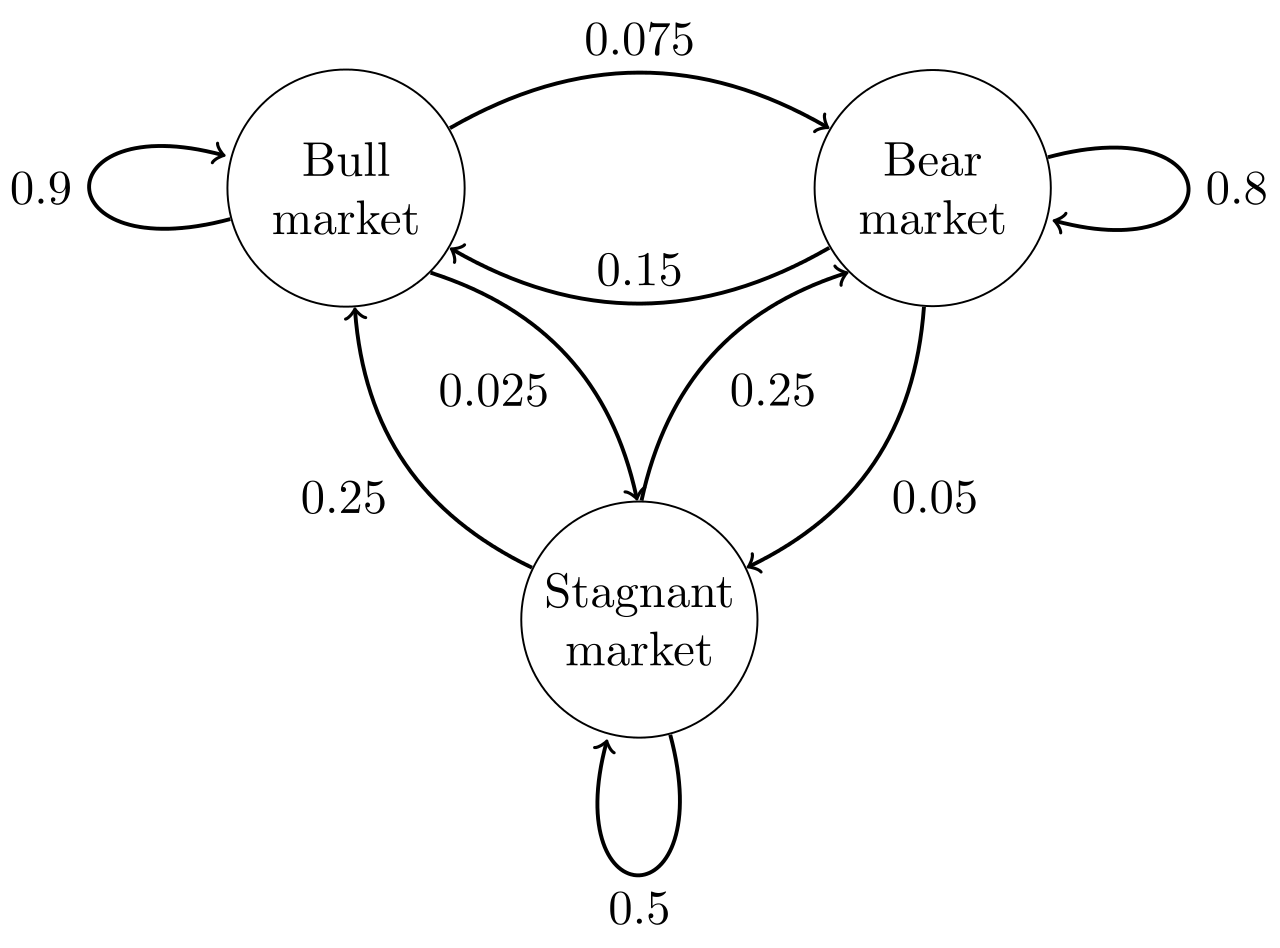
\includegraphics[width=0.5\textwidth]{StockMarket.png}
%\end{center}
%}


\end{document}
